\documentclass[11pt, reqno]{article}    % use "amsart" instead of "article" for AMSLaTeX format
\usepackage{my_packages}
\usepackage{tikz_packages}
\usepackage[american,siunitx]{circuitikz}
\usepackage{pgfplots}
\pgfplotsset{compat=1.14}
\usepackage[explicit]{titlesec}


\title{MAE 3145: PREDICT}
\author{Shankar Kulumani}
\date{Fall 2017}                          % Activate to display a given date or no date

\begin{document}
\begin{center}
{\Large \textbf{MAE3145: PREDICT}}
\end{center}
\subsection*{Description}
You are tasked to support teh elite Space Surveillance Reconstitution Team (SSRT) as an orbital analyst.
The SSRT will deploy to setup a remote space tracking capability when threat levels against the US indicate an attack in imminent.
As a SSRT member, it is your responsibility to develop software to locate satellite fom an Earth location.
In particular, SSRT's tacitcal terminal requires topocentric range, azimuth, and elevation to point its new secret tracking instruent.
Your program must compute and output this information at \underline{two minute intervals} each time the tactical \underline{terminal is in darkness} and the \underline{satellite is above the terminal's local horizon at a reasonable range}.
In addition, your program must determine if the statellite is visible to the tactical terminal, i.e. terminal in the dark, satellite illuminated by the sun, elevation angle greater than or equal to \SI{10}{\degree}, range less than \SI{1500}{\kilo\meter}.
If the satellite is in sunlight, SSRT members can operate teh terminal's new pointing instrument in one of three classified modes.

The SSRT's existence must be kept secret.
Thus, to validate your software \textbf{you must} view a low Earth orbiting satellite based on your program results.
In addition, if you know someone located at least \SI{100}{\kilo\meter} from our training site, and this person can be sworn to secrecy, give them your program results so they too can view a satellite.
Another person viewing a satellite based on yoru results will serve as a independent validation of your work.

As with all practical programming applications, there are three steps to this project:
\begin{enumerate}
    \item You will develop the correct algorithm and accomplish som hand calculations to provide a bsis to test your coded subroutines,
    \item You will code all subroutines, checking their output with that of your hand calculations to validate each subroutine as you go, eventually putting together the complete program and matching a provided single satellite data file perfectly,
    \item You will slightly alther this working program to accept a data file of hundres of real satellits, identify a viable vehicle to personally view, and go view it.
\end{enumerate}

The data required to run your program is located on \href{https://github.com/fdcl-gwu/MAE3145_library}{MAE3145: Astro Library}.
I will update these files throughout the semester.
The data comes from JSPOC's Two-Line Element Sets (TLEs), which are typically found in terms of three lines of data.
Each data set contains the 100+ brightest active payloads that JSPOC tracks.
However, not all satellites will be visible to the naked eye.

The TLE files are given in a very specifc format as shown in~\cref{fig:tle}. 
The following describes each paramerter contained in the TLEs.
Some of these numbers will not be used in your program. 
You may also get teh latest TLEs yourself at \href{www.clestrak.com}{celestrak.com}.
There are many references for the TLE description available in textbooks or online, but one is available \href{https://goo.gl/W6MZb2}{https://goo.gl/W6MZb2}.

\begin{figure}
    \centering
    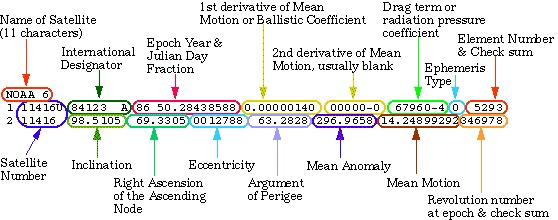
\includegraphics[width=\textwidth, keepaspectratio]{figures/tle.jpeg}
    \caption{TLE Format\label{fig:tle}}
\end{figure}
\subsection*{Project Requirements}
After completing the project you must submit the hard copies of your work:
\begin{itemize}
    \item Complete algorithms for the main driver script as well as a seperate algorithm for each sub-function that you develop.
        Someone totally unfamiliar with astrodynamics should be able to duplicate your program in any computer language.
    \item Clear, concise and properly documented and tested code
    \item Correct outputs from your program which matches the test cases
    \item Any additional test cases you may have used. 
        Explain why you did or did not use any additional test cases.
\end{itemize}

\subsection*{Authorized Resources}
You may consult with your instructor, the course notes or other reference material, and other students. 
However, you \textbf{MAY NOT} copy another student or any other individuals code. 
The program you develop must be your own work.

\subsection*{Algorithm}

Write a structured algorithm that shows your approach to writing a computer program to perform all of the tasks described above.
This should be a complete \textbf{sequential} list of the \textbf{equations and logic (including loop)} that you will use to write your program.
The details of subalgorithms are only required for procedures that are new for this project, not those provided to you.
Instead, just mention what procedure will be used and the inputs and outputs of the procedure, e.g. ``Calculate orbital elements given position and velocity vectors using \texttt{rv2coe}''.

When completed, anyone should be able to write your code \textbf{solely} using the algorithm in \textbf{any} computer language of their choice.
Thus, define all symbols before you use them, and do not write the equations and logic using any language specific terminology, i.e. Something like `` Find the length of the vector using \texttt{norm(x)} '' is unacceptable.

Your algorithm must be \textbf{typed}, which will serve you well when you document your final code. 
This is also a good opportunity to practice your technical writing skills in \LaTeX.

\subsection*{Final PREDICT Deliverables}

Your program must process the \texttt{PREDICT.DAT} data file and generate output that matches the orbital elements in \texttt{PREDICT.OUT} to at least four decimal places. 

Submit the following on the due date:
\begin{itemize}
    \item Fully documented driver script
    \item Each procedure which you wrote or modified, fully documented (no library routines)
    \item Computer generated results which match \texttt{PREDICT.OUT}
\end{itemize}

\subsection*{Program Specifications}
The following is a description of the required functions that your softwre program must include.
You will be making use of many of the functions that you have been developing over the course of the semester.

\subsubsection*{\texttt{J2Dragpert}}

This procedure calculates the rates of change of the right ascension of the ascending node, argument of periapsis, and eccentricty.
The perturbations considered are limited to \( J_2 \) and drag only.

\noindent \textbf{Inputs: }
\begin{itemize}
    \item \( i_0 \) - initial inclination in radians
    \item \( e_0 \) - initial eccentricty
    \item \( n_0 \) - initial mean motion in radians per second
    \item \( \frac{\dot{n}}{2} \) - mean motion rate divided by two in radians per second squared
\end{itemize}

\noindent\textbf{Output: }
\begin{itemize}
    \item \( \dot{\Omega} \) - nodal rate in radians per second
    \item \( \dot{\omega} \) - argument of periapsis rate in radians per second
    \item \( \dot{e} \) - eccentricity rate
\end{itemize}

\subsubsection*{Update}
This procedure uses the method of general perturbations to update the classical elements from \( t_0 \) to \( t_1 = t_0 + \delta t \) for inclined elliptical orbits.
It includes the effects due to first-order secular rates (second order for mean anomaly) caused by drag and Earth oblateness (\( J_2 \) ). 
It will be necessary to call \texttt{newton} from this function to calculate the future value of eccentric anomaly and true anomaly.

\noindent \textbf{Inputs: }
\begin{itemize}
    \item \( \delta t \) - elapsed time since \( t_0 \) in seconds
    \item \( n_0 \) - mean motion at \( t_0 \)
    \item \( \frac{\dot{n}}{2} \) - mean motion rate divided by 2
    \item \( e_0 \) - eccentricty at \( t_0 \)
    \item \( \dot{e} \) - eccentricity rate
    \item \( \Omega_0 \) - right ascension of the ascending node at \( t_0 \)
    \item \( \dot{\Omega}_0 \) - right ascension of the ascending node rate
    \item \( \omega_0 \) - argument of periapsis at \( t_0 \)
    \item \( \dot{\omega} \) - argument of periapsis rate
    \item \( M_0 \) - mean anomaly at \( t_0 \)
\end{itemize}

\noindent \textbf{Outputs:}

\begin{itemize}
    \item \( n \) - mean motion at \( t_1 \)
    \item \( e \) - eccentricty at \( t_1 \)
    \item \( \Omega \) - right ascension of the ascending node at \( t_1 \)
    \item \( \omega \) - arugment of periapsis at \( t_1 \)
    \item \( \nu \) - true anomaly at \( t_1 \)
\end{itemize}

\subsubsection*{\textbf{coe2rv}}
This function computes the spacecrafts position and velocity in the Earth centered inertial frame from the classical orbital elements.

\noindent \textbf{Inputs: }
\begin{itemize}
    \item \( n \) - mean motion at \( t_1 \)
    \item \( e \) - eccentricty at \( t_1 \)
    \item \( \Omega \) - right ascension of the ascending node at \( t_1 \)
    \item \( \omega \) - arugment of periapsis at \( t_1 \)
    \item \( \nu \) - true anomaly at \( t_1 \)
\end{itemize}

\noindent \textbf{Outputs: }
\begin{itemize}
    \item \( r \) -  position vector in ECI
    \item \( v \) - velocity vector in ECI
\end{itemize}

\subsubsection*{\textbf{visible} }
This function will determine if the observer is in the dark.
If so, it weill then compute the topocentric range, azimuth, and elevation of the satellite relative to the observer.
If the elevation is greater than \SI{10}{\degree} and the range is less than \SI{1500}{\kilo\meter} then the function will check if the satellite is illuminated by the sun.
If the satellite is visible then a flag will be set to true.

\noindent \textbf{Inputs: }
\begin{itemize}
    \item \( r \) -  position of the satellite in the ECI frame
    \item \( r_s \) - position of the observer in the ECI frame
    \item \( \lambda \) - observer geodetic latitude
    \item \( \theta \) - observer local sidereal time
    \item \( JD \) - julian date at viewing time
\end{itemize}

\noindent \textbf{Optional Outputs: }
\begin{itemize}
    \item \( \rho \) - range 
    \item \( \alpha \) - azimuth
    \item \( \epsilon \) - elevation
    \item \( d \) - flag for observer darkness
    \item \( v \) - flag for visibility of satellite
\end{itemize}

These outputs are all optional. 
You may decide to use this function to print your output data, or pass data to another function to output. 

\subsubsection*{rhoazel}
This function determines the topocentric range, azimuth, and elevation from the observation site to the satelite.

\noindent \textbf{Inputs: }
\begin{itemize}
    \item \(r \) -  position of satellite in ECI frame
    \item \( r_s \) - position of observer in ECI frame
    \item \( \lambda \) - observer geodetic latitude
    \item \( \theta \) - site local sidereal time
\end{itemize}

\noindent \textbf{Output: }
\begin{itemize}
    \item \( \rho \) - range
    \item \( \alpha \) - azimuth
    \item \( \epsilon \) - elevation
\end{itemize}

\subsection*{PREDICT Final Report}

Your program must process a TLE file and generate topocentric data so you can view a satellite.
You are required to summarize your project results and submit and engineering report (not to exceed \num{5} typed pages, excluding title page, table of contents and appendices) to your instructor.
Your report should contain the following sections:
\begin{enumerate}
    \item \textbf{Intro and Assumptions} - Introduce and motivate the problem, then briefly discuss the assumptions that were required to solve the problem. 
        You may simply list, without discussions, any assumptions being used that have been used in previous projects.
    \item \textbf{Math Technique} - This section is a summary of the theory that ws used to solve the problem, with an emphasis on the math that is new since \texttt{COMFIX}. 
        Be sure to address why each step was taken. 
        Do not discuss your computer code here, i.e. `` Next I wrote \texttt{rsite}\ldots'' and don't simply refer to or regurgiitate your algorithm.
    \item \textbf{Analysis/Discussion} - Introduce your code here and include a discussion of how it was validated, including options for validating.
        discuss teh output you generated, including a summary of the data on the satellite, or satellites) you viewed, along with details of that viewing as compared to what was expected.
    \item \textbf{Sources of Error/Recommendations} - Discuss any errors, that is, where your assumptions impacted your results. 
        Include any recommendations for how to improve the results.
    \item \textbf{Appendix A - Program Usage} - You must include instructions so a person can you your executable code to generate obsrevation data for any site, range of days, and any number of TLEs.
        Write this section of your report as \textbf{if it were a page in a user's manual}.
        Begin by briefly saying what your program does.
        Describe how someone would use your program.
        Are there any limits, e.g. matrix size or range of values?
        Is there anything unique to your program?
        Are there any data for which teh program will not work?
        As an example here's a good format you can use:
        \begin{itemize}
            \item Program Name
            \item Program function
            \item Computer used/limits
            \item Language and version
            \item How to run it
            \item Input
                \begin{itemize}
                    \item What are your inputs/units/limits?
                    \item What method is used to input the data, i.e. how do you change the input data?
                    \item Point out user interactive prompts if there are any.
                \end{itemize}
            \item Output
                \begin{itemize}
                    \item Explain the method used to output the data?
                    \item What are your outputs/units?
                \end{itemize}
        \end{itemize}
    \item \textbf{Appendix B - Results} - Program results for atleast 3 objects from teh TLEs (\textbf{NOT ALL 100+ please!}), over the time interval of your choice, to include when you observed a satellite.
    \item \textbf{Appendix C - Bonus} - Pick a location more than \SI{100}{\kilo\meter} from DC and run your program. 
        If you or any other person view a satellite based on your computer results, you will receive a bonus on your project
\end{enumerate}
\end{document}  
